\documentclass{bioinfo}
\copyrightyear{2025} \pubyear{2025}



% tightlist command for lists without linebreak
\providecommand{\tightlist}{%
  \setlength{\itemsep}{0pt}\setlength{\parskip}{0pt}}




% hyperref makes the margins screwy.
% https://groups.google.com/forum/#!topic/latexusersgroup/4W_SwGk6zx4
% http://ansuz.sooke.bc.ca/software/latex-tricks.php
% \usepackage[colorlinks=true, allcolors=blue]{hyperref}

\access{Advance Access Publication Date:   }
\appnotes{Application Note}

\begin{document}


\firstpage{1}

\subtitle{Genome analysis}

\title[Bioinformatics Rmd Template]{faers: An R Package for Seamlessly
Bridging the FAERS Database to R and Delivering Unified
Pharmacovigilance Workflows}

\author[FirstAuthorLastName \textit{et~al}.]{
Shixiang Wang\,\textsuperscript{1}, Yun
Peng\,\textsuperscript{2}, Zhangyu Wang\,\textsuperscript{1}
}

\address{
\textsuperscript{1}Central South University\\
\textsuperscript{2}aaa\\
}

\corresp{To whom correspondence should be addressed. E-mail: qq}

\history{Received on XXX; revised on XXX; accepted on XXX}

\editor{Associate Editor: XXX}

\abstract{
\textbf{Motivation:} The FDA Adverse Event Reporting System (FAERS)
serves as a critical database for monitoring post-marketing drug
safety.However, the primary focus on safety signal detection within
FAERS has left a significant gap in integrating pharmacovigilance
analysis with genetic tools.Thus, we aim to effectively utilize FAERS
data to bridge pharmacovigilance with genetic analysis, thereby
enhancing the precision of safety assessments and facilitating the
development of personalized medicine approaches.\\
\textbf{Results:} We developed the R package faers, which seamlessly
connects the FAERS database to the R programming language and provides a
unified approach for the seamless execution of pharmacovigilance
analysis and the integration of genetic tools in R.\\
\textbf{Availability:} faers is available on CRAN and on GitHub at
(https://github.com/Yunuuuu/faers).\\
\textbf{Contact:}212@qq.com\\
\textbf{Supplementary information:} Supplementary data are available at
Bioinformatics Online.}

\maketitle

\section{Introduction}

Cite others using bracket notation \citep{pepe2003statistical}. Can also
cite with \citet{zou2005regularization}.

The FDA Adverse Event Reporting System (FAERS) is the core database for
post-marketing safety monitoring of all approved drugs and therapeutic
biologics by the FDA. As required by regulations, it consolidates
mandatory adverse event reports submitted by pharmaceutical companies,
as well as voluntary first-hand information reported by individuals and
healthcare professionals. The data, which has been collected since
January 2004 and is continuously updated on a quarterly basis, includes
eight types of documents: demographic and administrative information,
detailed drug information, indications for use, report sources, drug
start and end dates, patient outcomes, reports of therapeutic failure,
and adverse events. Its core value is reflected in key areas such as
early safety signal detection, risk assessment, and drug labeling
revisions, providing direct evidence for the FDA to formulate drug
safety policies and risk management measures.

Introduce your topic. Lorem ipsum ad nauseum. Introduce your topic.
Lorem ipsum ad nauseum. Introduce your topic. Lorem ipsum ad nauseum.
Introduce your topic. Lorem ipsum ad nauseum. Introduce your topic.
Lorem ipsum ad nauseum.

Introduce your topic. Lorem ipsum ad nauseum. Introduce your topic.
Lorem ipsum ad nauseum. Introduce your topic. Lorem ipsum ad nauseum.
Introduce your topic. Lorem ipsum ad nauseum. Introduce your topic.
Lorem ipsum ad nauseum.

\section{Approach}

Here is how to include math equations in the document (bounded by
\texttt{\$\$}):

\[
\begin{aligned}
(x+y)^3&=(x+y)(x+y)^2\\
       &=(x+y)(x^2+2xy+y^2) \label{eqn:example} \\
       &=x^3+3x^2y+3xy^3+x^3. 
\end{aligned}
\]

Describe the approach. Lorem ipsum ad nauseum. Introduce your topic.
Lorem ipsum ad nauseum. Introduce your topic. Lorem ipsum ad nauseum.
Introduce your topic. Lorem ipsum ad nauseum. Introduce your topic.
Lorem ipsum ad nauseum.

Describe the approach. Lorem ipsum ad nauseum. Introduce your topic.
Lorem ipsum ad nauseum. Introduce your topic. Lorem ipsum ad nauseum.
Introduce your topic. Lorem ipsum ad nauseum. Introduce your topic.
Lorem ipsum ad nauseum.

Describe the approach. Lorem ipsum ad nauseum. Introduce your topic.
Lorem ipsum ad nauseum. Introduce your topic. Lorem ipsum ad nauseum.
Introduce your topic. Lorem ipsum ad nauseum. Introduce your topic.
Lorem ipsum ad nauseum.

Describe the approach. Lorem ipsum ad nauseum. Introduce your topic.
Lorem ipsum ad nauseum. Introduce your topic. Lorem ipsum ad nauseum.
Introduce your topic. Lorem ipsum ad nauseum. Introduce your topic.
Lorem ipsum ad nauseum.

\begin{figure}
\centering
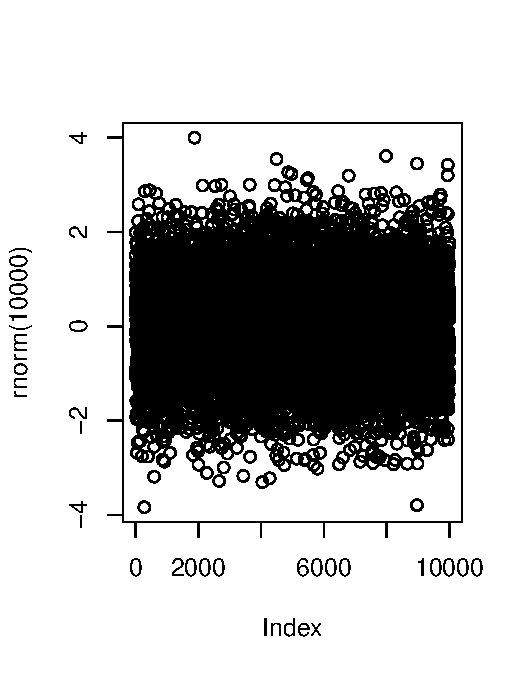
\includegraphics{faers_files/figure-latex/figure-1.pdf}
\caption{Figure from an Rmd chunk.}
\end{figure}

\section{Methods}

Detailed methods. Lorem ipsum ad nauseum. Introduce your topic. Lorem
ipsum ad nauseum. Introduce your topic. Lorem ipsum ad nauseum.
Introduce your topic. Lorem ipsum ad nauseum. Introduce your topic.
Lorem ipsum ad nauseum.

Detailed methods. Lorem ipsum ad nauseum. Introduce your topic. Lorem
ipsum ad nauseum. Introduce your topic. Lorem ipsum ad nauseum.
Introduce your topic. Lorem ipsum ad nauseum. Introduce your topic.
Lorem ipsum ad nauseum.

Detailed methods. Lorem ipsum ad nauseum. Introduce your topic. Lorem
ipsum ad nauseum. Introduce your topic. Lorem ipsum ad nauseum.
Introduce your topic. Lorem ipsum ad nauseum. Introduce your topic.
Lorem ipsum ad nauseum.

\subsection{Sub-Method}

Details for Method 1. Lorem ipsum ad nauseum. Introduce your topic.
Lorem ipsum ad nauseum. Introduce your topic. Lorem ipsum ad nauseum.
Introduce your topic. Lorem ipsum ad nauseum. Introduce your topic.
Lorem ipsum ad nauseum.

Details for Method 1. Lorem ipsum ad nauseum. Introduce your topic.
Lorem ipsum ad nauseum. Introduce your topic. Lorem ipsum ad nauseum.
Introduce your topic. Lorem ipsum ad nauseum. Introduce your topic.
Lorem ipsum ad nauseum.

Details for Method 1. Lorem ipsum ad nauseum. Introduce your topic.
Lorem ipsum ad nauseum. Introduce your topic. Lorem ipsum ad nauseum.
Introduce your topic. Lorem ipsum ad nauseum. Introduce your topic.
Lorem ipsum ad nauseum.

Details for Method 1. Lorem ipsum ad nauseum. Introduce your topic.
Lorem ipsum ad nauseum. Introduce your topic. Lorem ipsum ad nauseum.
Introduce your topic. Lorem ipsum ad nauseum. Introduce your topic.
Lorem ipsum ad nauseum.

\subsection{Method 2}

Details for Method 2. Lorem ipsum ad nauseum. Introduce your topic.
Lorem ipsum ad nauseum. Introduce your topic. Lorem ipsum ad nauseum.
Introduce your topic. Lorem ipsum ad nauseum. Introduce your topic.
Lorem ipsum ad nauseum.

Details for Method 2. Lorem ipsum ad nauseum. Introduce your topic.
Lorem ipsum ad nauseum. Introduce your topic. Lorem ipsum ad nauseum.
Introduce your topic. Lorem ipsum ad nauseum. Introduce your topic.
Lorem ipsum ad nauseum.

Details for Method 2. Lorem ipsum ad nauseum. Introduce your topic.
Lorem ipsum ad nauseum. Introduce your topic. Lorem ipsum ad nauseum.
Introduce your topic. Lorem ipsum ad nauseum. Introduce your topic.
Lorem ipsum ad nauseum.

Details for Method 2. Lorem ipsum ad nauseum. Introduce your topic.
Lorem ipsum ad nauseum. Introduce your topic. Lorem ipsum ad nauseum.
Introduce your topic. Lorem ipsum ad nauseum. Introduce your topic.
Lorem ipsum ad nauseum.

\section{Discussion}

Discussion of results. Lorem ipsum ad nauseum. Introduce your topic.
Lorem ipsum ad nauseum. Introduce your topic. Lorem ipsum ad nauseum.
Introduce your topic. Lorem ipsum ad nauseum. Introduce your topic.
Lorem ipsum ad nauseum.

Discussion of results. Lorem ipsum ad nauseum. Introduce your topic.
Lorem ipsum ad nauseum. Introduce your topic. Lorem ipsum ad nauseum.
Introduce your topic. Lorem ipsum ad nauseum. Introduce your topic.
Lorem ipsum ad nauseum.

Discussion of results. Lorem ipsum ad nauseum. Introduce your topic.
Lorem ipsum ad nauseum. Introduce your topic. Lorem ipsum ad nauseum.
Introduce your topic. Lorem ipsum ad nauseum. Introduce your topic.
Lorem ipsum ad nauseum.

Discussion of results. Lorem ipsum ad nauseum. Introduce your topic.
Lorem ipsum ad nauseum. Introduce your topic. Lorem ipsum ad nauseum.
Introduce your topic. Lorem ipsum ad nauseum. Introduce your topic.
Lorem ipsum ad nauseum.

\section{Conclusion}

Anything else? Lorem ipsum ad nauseum. Introduce your topic. Lorem ipsum
ad nauseum. Introduce your topic. Lorem ipsum ad nauseum. Introduce your
topic. Lorem ipsum ad nauseum. Introduce your topic. Lorem ipsum ad
nauseum.

Anything else? Lorem ipsum ad nauseum. Introduce your topic. Lorem ipsum
ad nauseum. Introduce your topic. Lorem ipsum ad nauseum. Introduce your
topic. Lorem ipsum ad nauseum. Introduce your topic. Lorem ipsum ad
nauseum.

Anything else? Lorem ipsum ad nauseum. Introduce your topic. Lorem ipsum
ad nauseum. Introduce your topic. Lorem ipsum ad nauseum. Introduce your
topic. Lorem ipsum ad nauseum. Introduce your topic. Lorem ipsum ad
nauseum.

Anything else? Lorem ipsum ad nauseum. Introduce your topic. Lorem ipsum
ad nauseum. Introduce your topic. Lorem ipsum ad nauseum. Introduce your
topic. Lorem ipsum ad nauseum. Introduce your topic. Lorem ipsum ad
nauseum.

\section*{Acknowledgements}
\addcontentsline{toc}{section}{Acknowledgements}

These should be included at the end of the text and not in footnotes.
Please ensure you acknowledge all sources of funding, see funding
section below.

Details of all funding sources for the work in question should be given
in a separate section entitled `Funding'. This should appear before the
`Acknowledgements' section.

\section*{Funding}
\addcontentsline{toc}{section}{Funding}

The following rules should be followed:

\begin{itemize}
\tightlist
\item
  The sentence should begin: `This work was supported by \ldots{}' -
\item
  The full official funding agency name should be given, i.e.~`National
  Institutes of Health', not `NIH' (full RIN-approved list of UK funding
  agencies)
\item
  Grant numbers should be given in brackets as follows: `{[}grant number
  xxxx{]}'
\item
  Multiple grant numbers should be separated by a comma as follows:
  `{[}grant numbers xxxx, yyyy{]}'
\item
  Agencies should be separated by a semi-colon (plus `and' before the
  last funding agency)
\item
  Where individuals need to be specified for certain sources of funding
  the following text should be added after the relevant agency or grant
  number `to {[}author initials{]}'.
\end{itemize}

An example is given here: `This work was supported by the National
Institutes of Health {[}AA123456 to C.S., BB765432 to M.H.{]}; and the
Alcohol \& Education Research Council {[}hfygr667789{]}.'

Oxford Journals will deposit all NIH-funded articles in PubMed Central.
See Depositing articles in repositories -- information for authors for
details. Authors must ensure that manuscripts are clearly indicated as
NIH-funded using the guidelines above.


% Bibliography
\bibliographystyle{natbib}
\bibliography{bibliography.bib}

\end{document}
